\subsection{Problem 6}%
\label{sec:problem_6}
Using least squares techniques, fit the following data
\begin{center}
  \begin{tabular}{|c|c|c|c|c|c|c|c|c|c|c|c|}
    \hline
    $x_i$ & -5 & -4 & -3 & -2 & -1 & 0 & 1 & 2 & 3 & 4 & 5 \\
    \hline
    $y_i$ & 2 & 7 & 9 & 12 & 13 & 14 & 14 & 13 & 10 & 8 & 4 \\
    \hline
  \end{tabular}
\end{center}
with a line $y=a_0+a_1x$ and then fit the data with a quadratic $y=a_0+a_1x+a_2x^2$.
Determine which of these two curves best fits the data by computing the $l_2$ norm of
the errors in each case.
%%%%%%%%%%%%%%%%%%%%%%%%%%%%%%%%%%%%%%%%%%%%%%%%%%%%%%%%%%%%%%%%%%%%%%%%%%%%%%%
\subsubsection*{Solution}
%%%%%%%%%%%%%%%%%%%%%%%%%%%%%%%%%%%%%%%%%%%%%%%%%%%%%%%%%%%%%%%%%%%%%%%%%%%%%%%
Finding a solution to this problem is a straightforward continuation of the previous
ones.
\lstinputlisting[style=Matlab-editor]{problems/Problem_6.m}
\begin{figure}
  \centering
  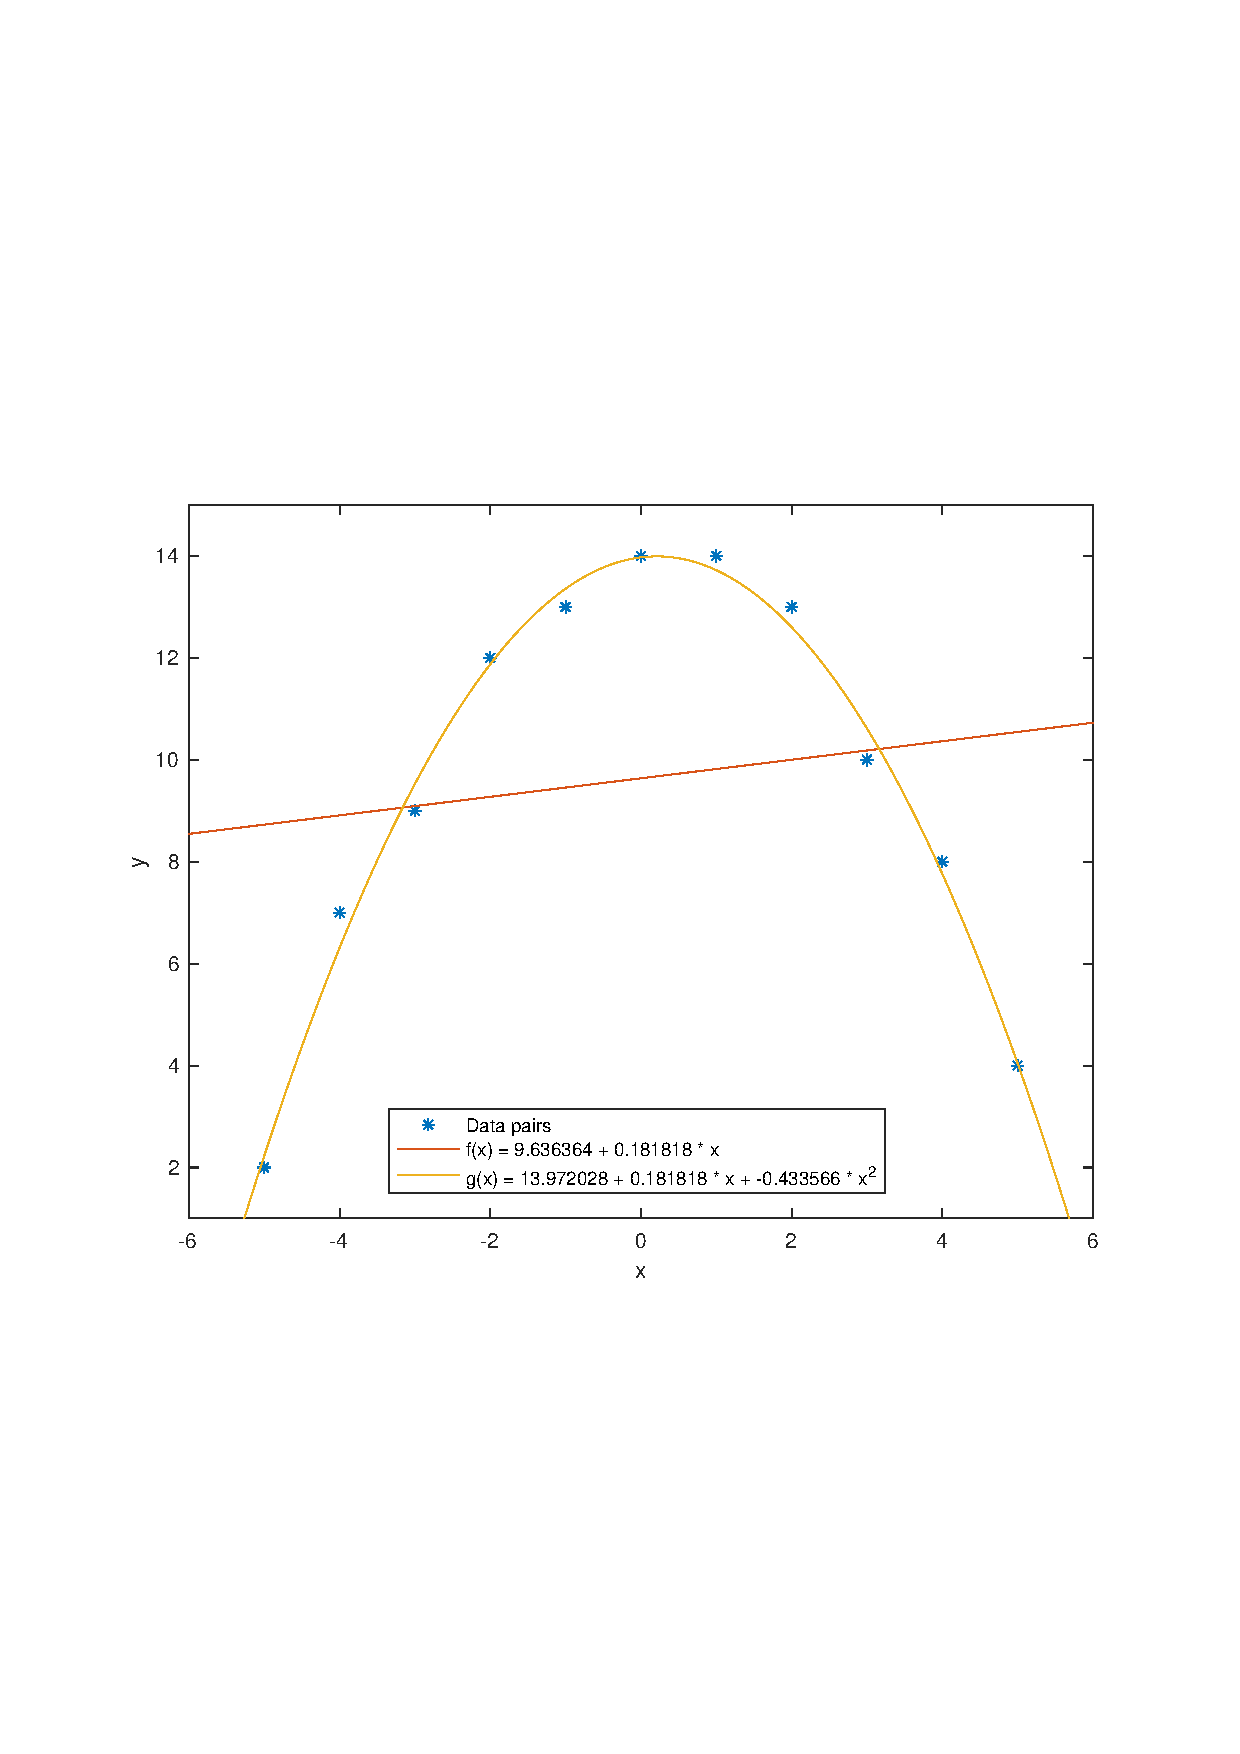
\includegraphics[width=0.7\textwidth]{images/Problem_6_plot.pdf}
  \caption{The plot of the data points from the Problem 6, approximated with the linear
    regression with $\varepsilon = 12.7636$ and the quadratic regression with
    $\varepsilon = 1.2737$.}
  \label{fig:problem_6}
\end{figure}

Both regressions are plotted in the~\autoref{fig:problem_6}, which shows he quadratic
equation nicely fits the data points, as expected from its lower error.
